\documentclass[]{article}

\usepackage{listings}
\usepackage{amsmath}
\usepackage{algorithm}
\usepackage[noend]{algpseudocode}
\usepackage{amssymb}
\usepackage{graphicx}
\usepackage{setspace}
\usepackage{pdfpages}
\usepackage{enumitem}
\lstset{language=Python}

\title{Operating Systems : Lab 1}
\author{Sean Noran}

\begin{document}

\maketitle

\onehalfspacing

\section{Sample Output}

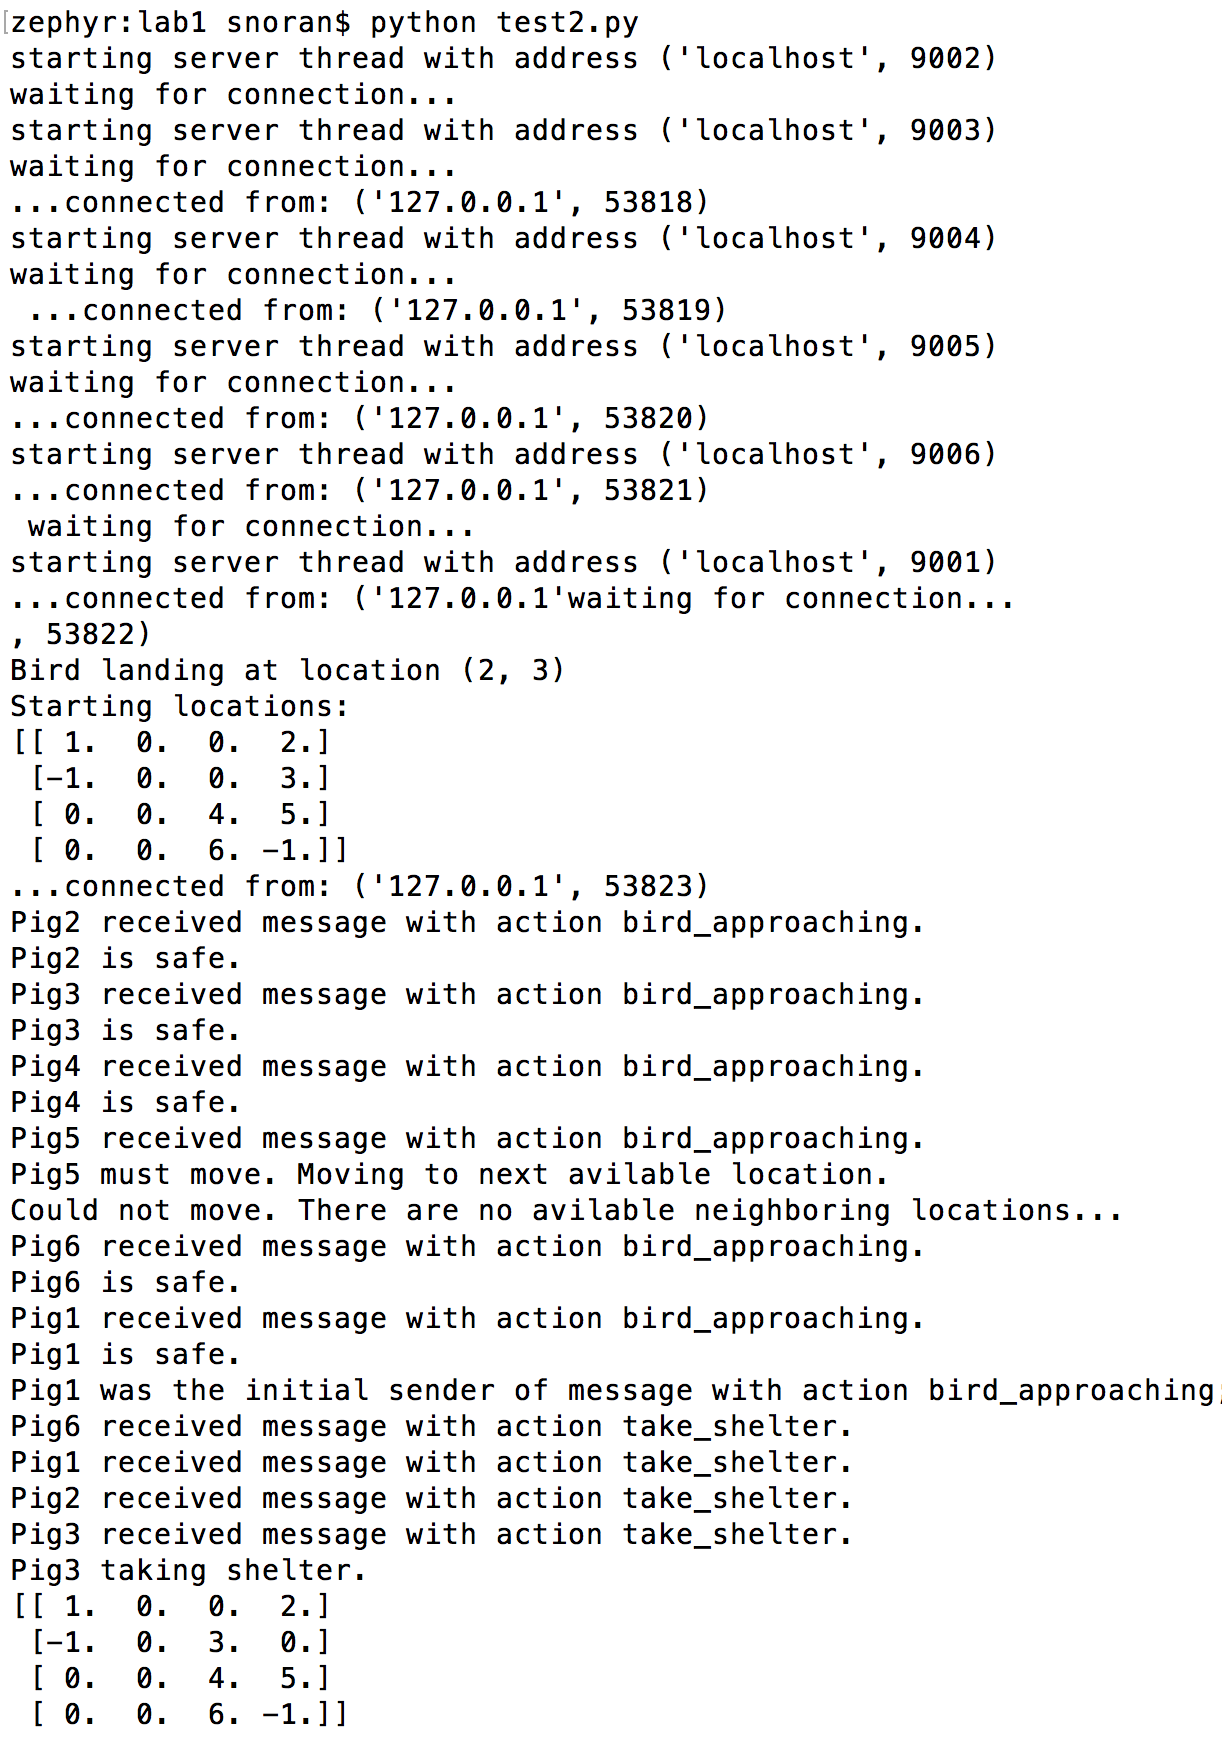
\includegraphics[scale=0.5]{output}

\section{Design}

\subsection{P2PNode Implementation}

The application was written in Python. Pigs inherit from a base P2PNode class, which is a node in a generic bidirectional socket-based peer-to-peer network. The P2PNode class has a connect() method, which accepts as parameter the node to connect to; in other words, the node passed in as a parameter acts as a server to which the current node instance can connect as a client. This is done by starting a server thread on the peer, which asynchronously binds to the host and listens on the port for connection requests. The client node then connects after a small but sufficient nodeN.connect(node1), we can generate a circular peer-to-peer network. I chose for the last node to connect back to the first so that any one-way communication can be assured to reach all nodes in the network and message propagation can be terminated easily by checking the sender's node ID against the current ID.

Message passing is done by populating two thread-safe queues, one associated with each direction of communication. By convention, I call the backward direction a "response". The send\_message(), which simply adds the message to the appropriate queue, also accepts an optional direction parameter, which by default is "forward", but can also be set to "backward". The message queue is then drained through the client socket and the response queue is drained into the server socket. Messages are, by convention, JSON strings, which can parsed to Python dictionaries very easily.

Messages are then passed to the on\_message\_received() callback defined in the P2PNode class. It is an empty method stub which is meant to be overridden by subclasses of the P2PNode class, e.g. the Pig class. More specifically, P2P nodes should know nothing about the details of pigs. I more or less opted for the object-oriented approach.

\subsection{Pig Implementation}

The Pig class is a subclass of P2PNode with some additional pig-specific functionality. When initializing a pig, an address and grid location must be specified, and there is an additional send\_delay parameter, which indicates how many seconds should wait before messages are sent to P2PNodes. The on\_message\_received() function overrides its superclass method and handles messages sent by other pigs.

Messages are fairly standard: They have a 'sender' field to identify which pigs sent the message initially; this ensures that responses to requests arrive at the requesting pig and that messages propagated through the entire network do not propagate indefinitely (since it's circular!). The 'action' field identifies what kind of message it is, e.g. 'request\_status' or 'take\_shelter'. The 'propagate' method indicates whether or not the message should propagate through the P2P network; this is probably an unnecessary field, since in all cases this field is True. Messages also have a 'hop\_count' field indicating how far it can propagate. And then there are the action-specific fields, such as the 'pigID' field when requesting a particular pig's status.

The other pig methods are based off this messaging protocol and only construct and send the initial message. These include broadcast\_bird\_approaching(), which requires a location at which the bird lands. The actions taken by pigs receiving this method execute in the on\_message\_received() method. The same holds for take\_shelter(), request\_status() and request\_status\_all().

This means that the on\_message\_received() method is quite bloated, which several nested if-else clauses. This can easily be improved by organizing this functionality in different methods and calling them in a switch statement on the message's 'action' field.

\subsection{Constructing Pig Network}

Based on the object-oriented design described above, it's very simple to create a pig-to-pig network.

\begin{lstlisting}
location = (-1,-1) # initial coordinates outside of the grid to ensure we enter the generation loop
for i in range(n_pigs):
    pigID = 9001+i
    while location == (-1,-1) or grid[location] != 0:
        location = generate_random_coordinate(grid_size)
    grid[location] = i+1
    pigs.append(Pig(('localhost', pigID), location, 0))
\end{lstlisting}

This gives each pig a random coordinate within a predetermined grid and assigns a unique port on the local machine to each pig. I chose to employ this on localhost, but it could just as easily be distributed on different machines. Next, the pigs can be connected in a circular network as follows.

\begin{lstlisting}
# construct circular P2P network
prev_pig = pigs[0]
for pig in pigs[1:]:
    pig.set_open_neighbors(get_open_neighbors(pig.location))
    prev_pig.connect(pig)
    prev_pig = pig
prev_pig.connect(pigs[0])
\end{lstlisting}

Then when the bird is launched, a pig can notify other pigs in the network as follows.

\begin{lstlisting}
pigs[0].broadcast_bird_approaching(bird_landing)
\end{lstlisting}

The assignment details indicate that the pig closest to where the bird is launched should broadcast the bird's landing location, but since the bird's launching location is arbitrary, it is fair for an arbitrary pig to make that broadcast. Above, I selected the first pig, but this still works for any pig. Due to the circular nature of the P2P network, any pig can be the starting point of a message and it will propagate successfully to all pigs in the network.

The main thread, after the broadcast, will wait as many seconds as the bird's time of flight, allowing pigs to move out of the way as they are executing on separate threads. I do not define a trajectory, e.g. angle, or speed, since the speed is only used for computing the time of flight, which I figure is fair to assume is available, and the trajectory is only used for determining the landing location, which we also assumed is known with complete certainty by the pig broadcasting the location. Therefore, the bird\_landing and bird\_time\_of\_flight variables are used.

Once the bird lands, damage is calculated recursively in the main thread, starting at the bird's landing location. If that location is occupied by a pig, then that pig will receive 2 points of damage. Neighboring pigs receive 1 point of damage and neighboring stone pillars will collapse, impacting all their neighbors (damaging neighboring pigs by 1 or collapsing other stone pillars). I decided to give different damages if hit directly by the bird (2 points damage) or hit indirectly by another pig or pillar (1 point damage). Each pig has 10 points to start. Because I chose for pigs to have multiple points, the Pig class does not have a was\_hit(pigID, trueFlag) function; however, it does have the same functionality, by sending a message with 'action' = 'respond\_status'. Instead of returning a boolean flag indicating that it was hit, it simply returns its status. I found this to be preferable, because it allows for multiple hits per pig.

Also, each grid location can only be occupied by one entity. To ensure this each pig knows at the start what available neighboring locations there are. Locations are not available if they have another pig or a pillar occupying them. And of course, grid constraints must also be met. It is, therefore, possible that a pig is trapped and has no open adjacent locations, in which case it cannot move and will have to suffer any damage.

\section{Grid Output}

The grid is output as a NumPy array and should be straight-forward to understand. A $0$ indicates a free location; $-1$ indicates stone pillar; and all other positive integers correspond to pig IDs, starting at 1.

\section{Testing}

Running p2p.py will perform a simple test on the base P2P network. It creates two nodes, node1 and node2, on localhost:9001 and :9002 respectively. Node1 is connected to node2. First, node1 sends node2 a message with 'action' = 'test'. Then node2 sends the same message to node1, passing in direction="backward". Then node2 attempts to send the message forward, but has no node to send to. And lastly, node1 attempts to send the message backward and again has no node to send to. This works correctly as shown in the output below:

\begin{lstlisting}
Message received at address ('localhost', 9002).
Message received at address ('localhost', 9001).
no node to send to
no node to respond to
\end{lstlisting}

Now, let's get pigs involved. I set up the following grid in test1.py.

$\begin{array}{cccc}
1 & 0 & 0 & 2 \\
-1 & 0 & 0 & 3 \\
0 & 0 & 4 & 5 \\
0 & 0 & 6 & -1
\end{array}$
 
If the bird lands on location $(2,3)$, assuming the grid is zero-indexed, then pig $5$ should be hit. Pig $5$, having no where to move, must remain and suffer the damage. Assuming pig $5$ does NOT tell any other pigs to take shelter, we will expect pigs $3$ and $4$ to be hit and the pillar in the bottom-right corner to fall, damaging pig 6 as well. Thus, we expect the status of each pig after this scenario to be: (10, 10, 9, 9, 8, 9), which after the running the script is indeed the case.

If after being hit, however, pig 5 notifies pig 3 to take shelter, then pig 3 should be safe, giving an expected output of (10, 10, 10, 9, 8, 9), assuming that the message arrives at pig 3 in time. To ensure this, we can make sure the delay between the bird's landing and applying damage is significantly large enough, say 5 seconds. This test can be run in test2.py. The grid output now looks like this:
 
$\begin{array}{cccc}
1 & 0 & 0 & 2 \\
-1 & 0 & 3 & 0 \\
0 & 0 & 4 & 5 \\
0 & 0 & 6 & -1
\end{array}$
 
As is clear above, pig3 was able to move and its status is indeed 10 and not 9.

\section{Experiment}

If in test2.py, described above, the message propagation delay, defined in params.py, is modified to be 2 seconds, then the take\_shelter message will not propagate quickly enough from pig 5 to pig 3 and the grid output will be 

$\begin{array}{cccc}
1 & 0 & 0 & 2 \\
-1 & 0 & 0 & 3 \\
0 & 0 & 4 & 5 \\
0 & 0 & 6 & -1
\end{array}$
 
In this case, pig $3$ will suffer damage as a result of slow P2P communication.

Given the same configuration but where pig $4$ is located at location $(1,2)$ instead of $(2,2)$ (this is the commented-out value for pig\_locations in params.py), pig 5 now has the ability to move to avoid being hit by the bird. But only if it does so promptly, which of course is dependent on the P2P network communication speed and the time of flight of the bird. To test this, we can give the broadcasting job to different pigs and see whether it makes it to pig 5 in time.

With a propagation time of $2$ seconds and starting at pig $0$, the message clearly will not arrive at pig $5$ in time. To make sure that it doesn't move regardless after being hit by the bird, an impacted pig's available locations are reset to an empty list, making it unable to move. It doesn't make sense for it to be able to move because it has already been hit.

This is the grid output:

$\begin{array}{cccc}
1 & 0 & 0 & 2 \\
-1 & 0 & 0 & 3 \\
0 & 4 & 0 & 5 \\
0 & 0 & 6 & -1
\end{array}$
 
If, however, pig $3$ broadcasts the bird's landing (by commenting line $75$ and uncommenting line $76$ in test2.py),then pig $5$ is able to move in time:

$\begin{array}{cccc}
1 & 0 & 0 & 2 \\
-1 & 0 & 4 & 3 \\
0 & 0 & 5 & 0 \\
0 & 0 & 6 & -1
\end{array}$
 
This is because there are fewer P2P network links from pig $3$ to pig $5$ than from pig $1$ to pig $5$.

\end{document}